\documentclass{beamer}
\usetheme{Madrid}
\usecolortheme{default}
\usepackage{tikz}
\usetikzlibrary{shapes,arrows,positioning}
\usepackage{listings}
\usepackage{xcolor}
\usepackage{amsmath}
\usepackage{amssymb}

\lstset{
    basicstyle=\ttfamily\small,
    keywordstyle=\color{blue},
    commentstyle=\color{green!60!black},
    stringstyle=\color{red},
    breaklines=true
}
% Logo da instituição
\titlegraphic{
    \vspace{0.5cm}
    \includegraphics[width=0.075\textwidth]{logo.png}
}
\title{Abstração e Relacionamento de Entidades
Com Base em Problemas Reais}
\subtitle{NF1 - Análise e Desenvolvimento  de Sistmas}
\author{Prof. Me. Luis Vinicius Costa Silva}
\date{\today}

\begin{document}



\frame{\titlepage}

\begin{frame}{O que veremos na aula de hoje}

\begin{itemize}
    \item ACID
    \item Modelo Entidade–Relacionamento (MER)
        \begin{itemize}
            \item Entidades, atributos e relacionamentos
            \item Cardinalidade (mínima e máxima)
            \item Entidade fraca e relacionamento identificador
            \item Generalização e entidade associativa
        \end{itemize}
        
    \item Do MER ao Modelo Relacional
        \begin{itemize}
            \item Tabelas, chaves primária e estrangeira
            \item Integridade referencial
            \item Transposição DER → Tabelas
        \end{itemize}
        
    \item Qualidade do Projeto
        \begin{itemize}
            \item Dependência funcional
            \item Formas Normais
        \end{itemize}
        
    \item Manipulação Formal de Dados
        \begin{itemize}
            \item Álgebra Relacional
            \item Cálculo Relacional
        \end{itemize}
\end{itemize}

\end{frame}









%=================================================
\section{ACID no Banco Company}





%-
\begin{frame}{ACID – Conceito Geral}

ACID define propriedades fundamentais das transações em bancos relacionais.

\begin{itemize}
    \item \textbf{A} — Atomicidade
    \item \textbf{C} — Consistência
    \item \textbf{I} — Isolamento
    \item \textbf{D} — Durabilidade
\end{itemize}

Garantem:
\begin{itemize}
    \item Segurança
    \item Integridade dos dados
    \item Confiabilidade do sistema
\end{itemize}

\end{frame}






%-
\begin{frame}[fragile]{Atomicidade (Atomicity)}

\textbf{Princípio:}
Uma transação ocorre por completo ou não ocorre.

\textbf{Exemplo no Company:}

Transferir empregado para outro departamento:

\begin{verbatim}
BEGIN;

UPDATE Empregado
SET DNUM = 3
WHERE NSS = 10;

UPDATE Departamento
SET TotalEmpregados = TotalEmpregados + 1
WHERE Dnumero = 3;

COMMIT;
\end{verbatim}

Se uma das operações falhar → ROLLBACK.

\end{frame}





%-
\begin{frame}{Problema sem Atomicidade}

Imagine:

\begin{itemize}
    \item Empregado mudou de departamento
    \item Contador do departamento não foi atualizado
\end{itemize}

Resultado:
\begin{itemize}
    \item Dados inconsistentes
    \item Informações incorretas para relatórios
\end{itemize}

Atomicidade impede esse cenário.

\end{frame}







%-
\begin{frame}{Consistência (Consistency)}

\textbf{Princípio:}
O banco deve sempre respeitar as regras definidas.

Exemplos no Company:

\begin{itemize}
    \item FK DNUM deve existir em Departamento
    \item PK NSS não pode repetir
    \item Horas em Trabalha\_em não pode ser negativa
\end{itemize}

Após COMMIT:
\begin{itemize}
    \item Todas as restrições continuam válidas
\end{itemize}

\end{frame}





%-
\begin{frame}[fragile]{Violação de Consistência}

\begin{verbatim}
INSERT INTO Empregado (NSS, DNUM)
VALUES (20, 999);
\end{verbatim}

Se não existir Departamento 999:

→ Erro de integridade referencial  
→ Transação é abortada

\end{frame}







%-
\begin{frame}{Isolamento (Isolation)}

\textbf{Princípio:}
Transações simultâneas não devem interferir incorretamente.

Exemplo:

Transação A:
\begin{itemize}
    \item Atualiza salário de um empregado
\end{itemize}

Transação B:
\begin{itemize}
    \item Consulta média salarial
\end{itemize}

Sem isolamento:
\begin{itemize}
    \item Pode ocorrer leitura suja (dirty read)
\end{itemize}

\end{frame}





%-
%\begin{frame}{Níveis de Isolamento}

%Principais níveis:

%\begin{itemize}
%    \item Read Uncommitted
%    \item Read Committed
%    \item Repeatable Read
%    \item Serializable
%\end{itemize}

%\textbf{Serializable:}
%Simula execução sequencial das transações.

%Mais seguro, porém mais custoso.

%\end{frame}







%-
\begin{frame}{Durabilidade (Durability)}

\textbf{Princípio:}
Após COMMIT, os dados não podem ser perdidos.

Exemplo:

\begin{verbatim}
UPDATE Empregado
SET Salario = 8000
WHERE NSS = 5;

COMMIT;
\end{verbatim}

Mesmo que:
\begin{itemize}
    \item O servidor desligue
    \item Falte energia
\end{itemize}

A alteração permanece.

\end{frame}





%-
\begin{frame}{Como a Durabilidade é Garantida}

\begin{itemize}
    \item Write-Ahead Logging (WAL)
    \item Logs de transação
    \item Checkpoints
    \item Backup físico
\end{itemize}

Antes de gravar na tabela:
\begin{itemize}
    \item O log é gravado no disco
\end{itemize}

\end{frame}







%-
\begin{frame}{ACID aplicado ao Company}

\begin{itemize}
    \item Atomicidade → Transferência de empregado completa ou desfeita
    \item Consistência → FK e PK sempre válidas
    \item Isolamento → Atualizações simultâneas não geram erro lógico
    \item Durabilidade → Salário atualizado permanece após falha
\end{itemize}

Qual propriedade impede que um empregado fique associado a um departamento inexistente?

Resposta: Consistência.

\end{frame}



\begin{frame}{Questão – Associe as Situações às Propriedades ACID (Company)}

Associe corretamente as situações (Coluna A) às propriedades ACID (Coluna B):

\begin{columns}[T]

\column{0.55\textwidth}
\textbf{Coluna A – Situações}

\begin{enumerate}
    \item Um empregado é transferido de departamento, mas ocorre falha antes da atualização do novo setor.
    \item Após queda de energia, o salário atualizado continua armazenado no banco.
    \item Dois gerentes atualizam o salário do mesmo funcionário ao mesmo tempo sem gerar inconsistência.
    \item O sistema impede cadastrar um empregado em um departamento que não existe.
\end{enumerate}

\column{0.45\textwidth}
\textbf{Coluna B – Propriedades}

\begin{itemize}
    \item (A) Atomicidade
    \item (B) Consistência
    \item (C) Isolamento
    \item (D) Durabilidade
\end{itemize}

\end{columns}

\end{frame}

\begin{frame}{Gabarito – Propriedades ACID}

\begin{itemize}
    \item 1 – A (Atomicidade)
    \item 2 – D (Durabilidade)
    \item 3 – C (Isolamento)
    \item 4 – B (Consistência)
\end{itemize}

\vspace{0.5cm}

\textbf{Justificativa resumida:}

\begin{itemize}
    \item \textbf{Atomicidade:} operação completa ou totalmente desfeita.
    \item \textbf{Durabilidade:} dados persistem mesmo após falhas.
    \item \textbf{Isolamento:} concorrência não gera inconsistência.
    \item \textbf{Consistência:} regras de integridade (PK, FK, restrições) sempre válidas.
\end{itemize}

\end{frame}


%=================================================
\section{Modelo Entidade-Relacionamento}

%-------------------------------------------------
\begin{frame}{Entidade e Relacionamento}

\textbf{Entidade:}
\begin{itemize}
\item Objeto com existência própria.
\item Ex: Departamento, Empregado, Projeto.
\end{itemize}

\textbf{Relacionamento:}
\begin{itemize}
\item Associação entre entidades.
\item Ex: Empregado trabalha em Projeto.
\end{itemize}

\end{frame}

%-------------------------------------------------
\begin{frame}[fragile]{Entidade Forte → Tabela}

\begin{lstlisting}[language=SQL]
CREATE TABLE Departamento (
  Dnumero INTEGER UNSIGNED NOT NULL,
  DNome VARCHAR(20) NOT NULL,
  PRIMARY KEY(Dnumero)
);
\end{lstlisting}

\textbf{Por que é entidade forte?}
\begin{itemize}
\item Possui identificador próprio (Dnumero).
\item Não depende de outra entidade para existir.
\end{itemize}

\end{frame}

%-------------------------------------------------
\begin{frame}[fragile]{Auto-relacionamento}

Empregado supervisiona Empregado

\begin{lstlisting}[language=SQL]
CREATE TABLE Empregado (
  NSS INTEGER UNSIGNED NOT NULL,
  NSSSUPER INTEGER UNSIGNED,
  PRIMARY KEY(NSS),

  FOREIGN KEY (NSSSUPER)
  REFERENCES Empregado(NSS)
  -- FK aponta para a própria tabela
);
\end{lstlisting}

\textbf{Classificação:}
Auto-relacionamento binário 1:N

\end{frame}

%-------------------------------------------------
\begin{frame}[fragile]{Relacionamento 1:N}

Departamento (1) —— (N) Empregado

\begin{lstlisting}[language=SQL]
ALTER TABLE Empregado
ADD FOREIGN KEY (DNUM)
REFERENCES Departamento(Dnumero);
\end{lstlisting}

\textbf{Regra de transposição DER → Relacional:}
\begin{itemize}
\item PK do lado 1 vira FK no lado N.
\end{itemize}

\end{frame}

%-------------------------------------------------
\begin{frame}[fragile]{Relacionamento N:N}

Empregado trabalha em Projeto

\begin{lstlisting}[language=SQL]
CREATE TABLE Trabalha_em (
  NSSE INTEGER UNSIGNED NOT NULL,
  PNO INTEGER UNSIGNED NOT NULL,
  Horas INTEGER,
  PRIMARY KEY(NSSE, PNO)
);
\end{lstlisting}

\textbf{Observação:}
\begin{itemize}
\item Relacionamento N:N vira tabela associativa.
\item Pode possuir atributos (Horas).
\end{itemize}

\end{frame}

%=================================================
\section{Chaves e Integridade}

%-------------------------------------------------
\begin{frame}{Chave Primária (PK)}

\begin{itemize}
\item Identifica unicamente cada tupla.
\item Não pode repetir.
\item Não pode ser NULL.
\end{itemize}

Exemplo: NSS em Empregado.
\end{frame}

%-------------------------------------------------
\begin{frame}{Chave Estrangeira (FK)}

\begin{itemize}
\item Referencia PK de outra tabela.
\item Implementa relacionamentos.
\end{itemize}

\textbf{Integridade Referencial:}

FK deve existir na tabela referenciada.
\end{frame}

%-------------------------------------------------
\begin{frame}[fragile]{Exemplo de Integridade}

\begin{lstlisting}[language=SQL]
INSERT INTO Empregado (NSS, DNUM)
VALUES (1, 999);
-- Erro se não existir Departamento 999
\end{lstlisting}

\textbf{Questão típica de prova:}
Integridade referencial garante consistência entre FK e PK.
\end{frame}

%=================================================

%=================================================
\section{Álgebra Relacional}

%-------------------------------------------------


\begin{frame}{O que é Álgebra Relacional?}

\textbf{Álgebra Relacional} é uma linguagem procedural formal
para consultar bancos de dados relacionais.

\vspace{0.4cm}

\textbf{Características:}
\begin{itemize}
    \item Base matemática (Teoria dos Conjuntos)
    \item Define \textbf{operações} sobre relações (tabelas)
    \item Resultado de uma operação → outra relação
    \item Base teórica do SQL
\end{itemize}

\textbf{Ideia principal:}
"Como obter o resultado?"

\end{frame}





\begin{frame}{Principais Operadores da Álgebra Relacional}

\begin{itemize}
    \item $\sigma$ → Seleção (filtra linhas)
    \item $\pi$ → Projeção (seleciona colunas)
    \item $\times$ → Produto Cartesiano
    \item $\Join$ → Junção
    \item $-$ → Diferença
    \item $\cup$ → União
    \item $\div$ → Divisão
\end{itemize}

Cada operador transforma uma ou mais relações
em uma nova relação.

\end{frame}





\begin{frame}{Operador Seleção ($\sigma$)}

Filtra linhas com base em uma condição.

\textbf{Sintaxe:}
\[
\sigma_{condição}(Relação)
\]

\textbf{Exemplo:}
Empregados com salário maior que 5000:

\[
\sigma_{Salario > 5000}(Empregado)
\]

\textbf{Interpretação:}
Mantém apenas as tuplas que satisfazem a condição.

\end{frame}





\begin{frame}{Operador Projeção ($\pi$)}

Seleciona colunas específicas.

\textbf{Sintaxe:}
\[
\pi_{atributos}(Relação)
\]

\textbf{Exemplo:}
Listar apenas os nomes:

\[
\pi_{Pnome}(Empregado)
\]

\textbf{Importante:}
Remove colunas não especificadas
e elimina duplicatas.

\end{frame}





\begin{frame}{Composição de Operadores}

Problema:
Listar nomes de empregados com salário > 5000.

Passo 1: Selecionar
\[
\sigma_{Salario > 5000}(Empregado)
\]

Passo 2: Projetar
\[
\pi_{Pnome}(\sigma_{Salario > 5000}(Empregado))
\]

\textbf{Ordem importa!}

\end{frame}





\begin{frame}{Junção ($\Join$)}

Combina duas relações com base em uma condição.

\textbf{Sintaxe:}
\[
R \Join_{condição} S
\]

\textbf{Exemplo:}
Nome do empregado e nome do departamento:

\[
Empregado \Join_{DNUM=Dnumero} Departamento
\]

Depois projetamos:
\[
\pi_{Pnome, DNome}(...)
\]

\end{frame}





\begin{frame}{Produto Cartesiano ($\times$)}

Combina todas as tuplas de R com todas as tuplas de S.

\[
R \times S
\]

\textbf{Cuidado:}
Gera muitas combinações.

Normalmente usado como etapa intermediária
para definir junções.

\end{frame}





\begin{frame}{Diferença ($-$)}

Retorna tuplas que estão em uma relação
e não estão em outra.

\[
R - S
\]

\textbf{Exemplo:}
Empregados que não trabalham em projeto:

\[
\pi_{NSS}(Empregado) -
\pi_{NSSE}(Trabalha\_em)
\]

\end{frame}





\begin{frame}{Divisão ($\div$)}

Usada para consultas do tipo:
"para TODOS".

\[
R \div S
\]

\textbf{Exemplo:}
Empregados que trabalham em TODOS os projetos:

\[
\pi_{NSSE}(Trabalha\_em) \div
\pi_{PNumero}(Projeto)
\]

\end{frame}





\begin{frame}{O que é Cálculo Relacional?}

Linguagem declarativa formal.

\textbf{Não diz como obter o resultado.}
Diz apenas \textbf{o que deseja}.

Baseado em lógica de predicados.

\textbf{Duas formas:}
\begin{itemize}
    \item TRC – Cálculo Relacional de Tuplas
    \item DRC – Cálculo Relacional de Domínios
\end{itemize}

Base conceitual do SQL.

\end{frame}





\begin{frame}{TRC – Cálculo Relacional de Tuplas}

Forma geral:

\[
\{ t \mid Relação(t) \land condição(t) \}
\]

\textbf{Exemplo:}
Empregados com salário > 5000:

\[
\{ t \mid Empregado(t) \land t.Salario > 5000 \}
\]

\textbf{Leitura:}
Conjunto de tuplas t
tal que t pertence a Empregado
e satisfaz a condição.

\end{frame}





\begin{frame}{Álgebra vs Cálculo Relacional}

\begin{columns}

\column{0.5\textwidth}
\textbf{Álgebra Relacional}
\begin{itemize}
    \item Procedural
    \item Diz como fazer
    \item Base operacional
\end{itemize}

\column{0.5\textwidth}
\textbf{Cálculo Relacional}
\begin{itemize}
    \item Declarativo
    \item Diz o que quer
    \item Base lógica
\end{itemize}

\end{columns}

\vspace{0.4cm}

Ambos são equivalentes em poder expressivo.

\end{frame}



\begin{frame}{Operadores Fundamentais}

$\sigma$ (Seleção) → Filtra linhas  

$\pi$ (Projeção) → Seleciona colunas  

$\Join$ → Combina relações  

\end{frame}

%-------------------------------------------------
\begin{frame}[fragile]{Seleção em SQL}

\begin{lstlisting}[language=SQL]
SELECT *
FROM Empregado
WHERE Salario > 5000;
-- Corresponde a sigma
\end{lstlisting}

\end{frame}

%-------------------------------------------------
\begin{frame}[fragile]{Projeção em SQL}

\begin{lstlisting}[language=SQL]
SELECT Pnome
FROM Empregado;
-- Corresponde a pi
\end{lstlisting}

\end{frame}

%-------------------------------------------------
\begin{frame}{Exemplo}

$\pi_{Nome}(\sigma_{Curso='Computacao'}(Aluno))$

Passo 1: Seleciona alunos do curso  
Passo 2: Projeta apenas Nome  

Resposta correta: Seleção seguida de projeção.
\end{frame}

\begin{frame}{DER - Estrutura Principal}
\centering
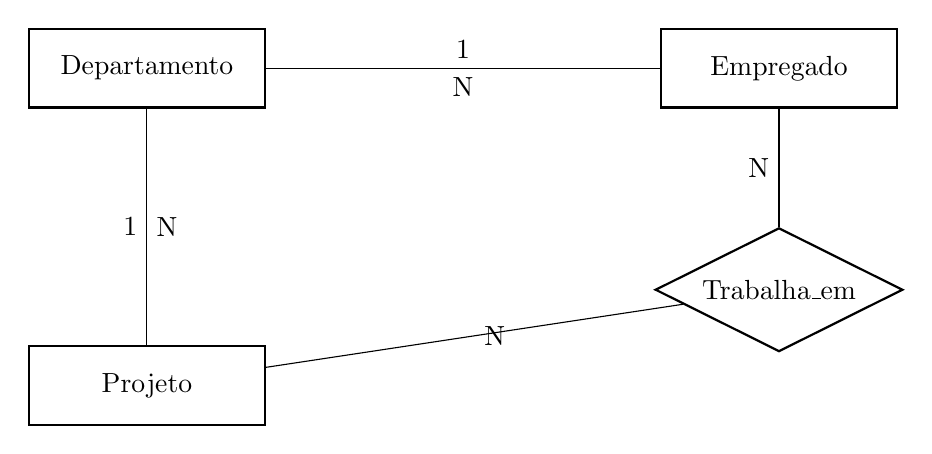
\begin{tikzpicture}[
entity/.style={rectangle, draw, thick, minimum width=3cm, minimum height=1cm},
relationship/.style={diamond, draw, thick, aspect=2},
attribute/.style={ellipse, draw},
]

% Entidades
\node[entity] (dep) {Departamento};
\node[entity, right=5cm of dep] (emp) {Empregado};
\node[entity, below=3cm of dep] (proj) {Projeto};

% Relacionamentos
\node[relationship, below=1.5cm of emp] (trab) {Trabalha\_em};

% Ligações Departamento - Empregado
\draw (dep) -- node[above]{1} node[below]{N} (emp);

% Ligações Departamento - Projeto
\draw (dep) -- node[left]{1} node[right]{N} (proj);

% Ligações Empregado - Trabalha_em - Projeto
\draw (emp) -- node[left]{N} (trab);
\draw (proj) -- node[right]{N} (trab);

\end{tikzpicture}
\end{frame}

%=================================================

\begin{frame}{Questão 1 -- Seleção}
Deseja-se listar os nomes dos empregados que possuem salário maior que 5000.

Qual das expressões abaixo representa corretamente essa consulta?
\end{frame}

\begin{frame}[fragile]{Questão 1 -- Gabarito}

\textbf{Resposta Correta}

\begin{columns}

\column{0.33\textwidth}
\textbf{Álgebra Relacional}

\[
\pi_{Pnome}
\big(\sigma_{Salario > 5000}(Empregado)\big)
\]

\column{0.33\textwidth}
\textbf{SQL}

\begin{verbatim}
SELECT Pnome
FROM Empregado
WHERE Salario > 5000;
\end{verbatim}

\column{0.33\textwidth}
\textbf{Cálculo Relacional (Tuplas)}

\[
\{\, e.Pnome \mid Empregado(e)
\wedge e.Salario > 5000 \,\}
\]

\end{columns}

\end{frame}

\begin{frame}{Como Chegar na Resposta}

\begin{itemize}
    \item Primeiro identificamos a tabela envolvida: Empregado
    \item Aplicamos a condição: Salario > 5000
    \item Projetamos apenas o atributo desejado (Pnome)
\end{itemize}

\begin{block}{Interpretação}
\begin{itemize}
    \item Álgebra: seleciona ($\sigma$) depois projeta ($\pi$)
    \item SQL: WHERE filtra, SELECT escolhe colunas
    \item Cálculo: define conjunto por predicado lógico
\end{itemize}
\end{block}

\end{frame}

\begin{frame}{Questão 2 -- Junção}
Liste o nome dos empregados e o nome do departamento onde trabalham.
\end{frame}


\begin{frame}[fragile]{Questão 2 -- Gabarito}

\begin{columns}

\column{0.33\textwidth}
\textbf{Álgebra Relacional}

\[
\pi_{Pnome, DNome}
\big(Empregado \bowtie_{DNUM = Dnumero} Departamento\big)
\]

\column{0.33\textwidth}
\textbf{SQL}

\begin{verbatim}
SELECT E.Pnome, D.DNome
FROM Empregado E
JOIN Departamento D
ON E.DNUM = D.Dnumero;
\end{verbatim}

\column{0.33\textwidth}
\textbf{Cálculo Relacional}

\[
\{\, e.Pnome, d.DNome \mid
Empregado(e) \wedge
Departamento(d) \wedge
e.DNUM = d.Dnumero \,\}
\]

\end{columns}

\end{frame}

\begin{frame}{Como Resolver}

\begin{itemize}
    \item Temos duas relações: Empregado e Departamento
    \item Condição de junção:
    \[
    e.DNUM = d.Dnumero
    \]
    \item Após a junção, projetamos apenas os atributos desejados
\end{itemize}

\begin{block}{Conceito Importante}
Junção é uma seleção sobre produto cartesiano
com condição de igualdade.
\end{block}

\end{frame}

\begin{frame}{Questão 3 -- Existência}
Liste os nomes dos projetos que possuem pelo menos um empregado trabalhando.
\end{frame}

\begin{frame}[fragile]{Questão 3 -- Gabarito}

\begin{columns}

\column{0.33\textwidth}
\textbf{Álgebra Relacional}

\[
\pi_{PNome}
\big(Projeto \bowtie_{PNumero = PNO} Trabalha\_em\big)
\]

\column{0.33\textwidth}
\textbf{SQL}

\begin{verbatim}
SELECT DISTINCT P.PNome
FROM Projeto P
JOIN Trabalha_em T
ON P.PNumero = T.PNO;
\end{verbatim}

\column{0.33\textwidth}
\textbf{Cálculo Relacional}

\[
\{\, p.PNome \mid Projeto(p)
\wedge \exists t \big(Trabalha\_em(t)
\wedge p.PNumero = t.PNO\big) \,\}
\]

\end{columns}

\end{frame}

%-------------------------------------------------
\begin{frame}{Pontos-Chave}

\begin{itemize}
\item Entidade fraca depende de entidade forte
\item 1:N → FK no lado N
\item N:N → tabela associativa
\item Integridade referencial garante consistência
\item 3FN elimina dependência transitiva
\item $\sigma$ = WHERE
\item $\pi$ = SELECT coluna
\end{itemize}

\end{frame}


\begin{frame}{Questão 1 – Álgebra Relacional}

Deseja-se listar os NOMES dos empregados
com salário maior que 5000.

Qual expressão está correta?

A) $\sigma_{Salario > 5000}(Empregado)$

B) $\pi_{Pnome}(\sigma_{Salario > 5000}(Empregado))$

C) $\pi_{Salario}(\sigma_{Pnome > 5000}(Empregado))$

D) $\sigma_{Pnome}(\pi_{Salario > 5000}(Empregado))$

E) $Empregado \Join Salario > 5000$

\end{frame}





\begin{frame}{Questão 1 – Gabarito}

Resposta correta:

\Large \textbf{B) $\pi_{Pnome}(\sigma_{Salario > 5000}(Empregado))$}

\end{frame}





\begin{frame}{Questão 1 – Explicação}

Passo 1: Interpretar o problema  
→ "salário maior que 5000" = FILTRAR linhas  
→ operador $\sigma$

Passo 2: Quer apenas o nome  
→ PROJETAR coluna Pnome  
→ operador $\pi$

Ordem correta:
1. Seleciona
2. Projeta

Erro comum:
Alternativa A filtra mas não retorna só os nomes.

\end{frame}









\begin{frame}{Questão 2 – Junção}

Listar nome do empregado e nome do departamento.

A) $\pi_{Pnome, DNome}(Empregado \Join Departamento)$

B) $\pi_{Pnome, DNome}(Empregado \Join_{DNUM=Dnumero} Departamento)$

C) $\sigma_{Pnome, DNome}(Empregado \times Departamento)$

D) $\pi_{Pnome}(Empregado) \Join Departamento$

E) $Empregado \times Departamento$

\end{frame}





\begin{frame}{Questão 2 – Gabarito}

Resposta correta:

\Large \textbf{B) $\pi_{Pnome, DNome}(Empregado \Join_{DNUM=Dnumero} Departamento)$}

\end{frame}





\begin{frame}{Questão 2 – Explicação}

Passo 1: São duas tabelas → precisa de junção.

Passo 2: Junção precisa de condição:
DNUM = Dnumero

Sem condição → produto cartesiano (errado).

Passo 3: Projetar apenas colunas desejadas.

Armadilha:
Alternativa A não especifica condição de junção.

\end{frame}







\begin{frame}{Questão 3 – Diferença}

Empregados que NÃO trabalham em projeto algum.

A) $\pi_{NSS}(Empregado) - \pi_{NSSE}(Trabalha\_em)$

B) $\pi_{NSSE}(Trabalha\_em) - \pi_{NSS}(Empregado)$

C) $Empregado \Join Trabalha\_em$

D) $\sigma_{NSSE=NULL}(Trabalha\_em)$

E) $\pi_{Pnome}(Trabalha\_em)$

\end{frame}





\begin{frame}{Questão 3 – Gabarito}

Resposta correta:

\Large \textbf{A) $\pi_{NSS}(Empregado) - \pi_{NSSE}(Trabalha\_em)$}

\end{frame}





\begin{frame}{Questão 3 – Explicação}

Ideia:
Total de empregados
MENOS
Empregados que aparecem em Trabalha_em.

Passo 1:
$\pi_{NSS}(Empregado)$

Passo 2:
$\pi_{NSSE}(Trabalha\_em)$

Passo 3:
Aplicar diferença.

Isso retorna os que não estão na segunda relação.

\end{frame}









\begin{frame}{Questão 4 – Divisão}

Empregados que trabalham em TODOS os projetos.

A) $Empregado \div Projeto$

B) $Trabalha\_em \div Projeto$

C) $\pi_{NSSE}(Trabalha\_em) \div \pi_{PNumero}(Projeto)$

D) $\pi_{PNumero}(Projeto) \div Trabalha\_em$

E) $Empregado \times Projeto$

\end{frame}





\begin{frame}{Questão 4 – Gabarito}

Resposta correta:

\Large \textbf{C) $\pi_{NSSE}(Trabalha\_em) \div \pi_{PNumero}(Projeto)$}

\end{frame}





\begin{frame}{Questão 4 – Explicação}

Divisão resolve:
"para TODOS".

Dividendo:
Trabalha_em (quem trabalha em quê)

Divisor:
Todos os projetos

Resultado:
Empregados que aparecem associados a todos os projetos.

\end{frame}









\begin{frame}{Questão 5 – TRC}

Empregados com salário maior que 5000:

A) $\{ t | Empregado(t) \land t.Salario > 5000 \}$

B) $\{ t.Pnome | Empregado(t.Salario > 5000) \}$

C) $\{ t | t \in Salario \land t > 5000 \}$

D) $\{ Empregado | Salario > 5000 \}$

E) $\{ t | t > 5000 \}$

\end{frame}





\begin{frame}{Questão 5 – Gabarito}

Resposta correta:

\Large \textbf{A)} $\{ t | Empregado(t) \land t.Salario > 5000 \}$

\end{frame}





\begin{frame}{Questão 5 – Explicação}

Estrutura do TRC:

\{ t | Relação(t) ∧ condição \}

Passo 1:
Definir variável de tupla (t)

Passo 2:
Dizer de qual relação ela vem

Passo 3:
Aplicar condição lógica

Outras alternativas quebram a sintaxe formal.

\end{frame}





%-------------------------------------------------
\begin{frame}
\centering
\Huge Dúvidas?
\end{frame}




\section{Normalização}

%-
\begin{frame}{O que é Normalização?}

Processo de organização das relações para:

\begin{itemize}
    \item Reduzir redundância
    \item Evitar anomalias (inserção, atualização, remoção)
    \item Garantir integridade lógica
\end{itemize}

Baseia-se em:
\begin{itemize}
    \item Dependências Funcionais
    \item Identificação correta de chaves
\end{itemize}

Objetivo:
Estruturar o esquema para evitar inconsistências.

\end{frame}





%-
\begin{frame}{Anomalias que a Normalização Evita}

\textbf{Anomalia de Inserção}

Não é possível cadastrar um departamento
sem ter um empregado associado.

\textbf{Anomalia de Atualização}

Alterar o nome do departamento exige
mudar em várias linhas.

\textbf{Anomalia de Remoção}

Excluir o último empregado pode apagar
informação do departamento.

\end{frame}





%-
\begin{frame}{Dependência Funcional}

Se A → B

A determina unicamente B.

Significa:
Para cada valor de A existe
apenas um valor possível de B.

Exemplos no Company:

\begin{itemize}
\item NSS → Pnome
\item NSS → Salario
\item DNUM → DNome
\end{itemize}

\end{frame}





%-
\begin{frame}{Chave Candidata}

Conjunto mínimo de atributos
que determina todos os demais.

Exemplo:

Empregado(NSS, Pnome, Salario, DNUM)

NSS → todos os outros atributos

Logo:
NSS é chave candidata.

\end{frame}





%-
\begin{frame}{Primeira Forma Normal (1FN)}

Regra:
\textbf{Atributos devem ser atômicos.}

Não pode haver:
\begin{itemize}
    \item Listas
    \item Conjuntos
    \item Valores repetidos em uma célula
\end{itemize}

Exemplo NÃO 1FN:

Empregado(NSS, Nome, Telefones)

Telefones = \{9999, 8888\}

Correção:
Criar relação Telefone(NSS, Numero)

\end{frame}





%-
\begin{frame}{Segunda Forma Normal (2FN)}

Requisito:
\begin{itemize}
    \item Estar na 1FN
    \item Não possuir dependência parcial
\end{itemize}

Dependência parcial:
Atributo depende de parte da chave composta.

Exemplo:

Trabalha\_em(NSS, PNumero, Horas, PNome)

Chave: (NSS, PNumero)

Se:
PNumero → PNome

Então há dependência parcial.

Solução:
Separar Projeto(PNumero, PNome)

\end{frame}





%-
\begin{frame}{Terceira Forma Normal (3FN)}

Requisito:
\begin{itemize}
    \item Estar na 2FN
    \item Não possuir dependência transitiva
\end{itemize}

Dependência transitiva:

A → B e B → C

Logo:
A → C (indiretamente)

Exemplo:

Empregado(NSS, Pnome, DNUM, DNome)

Se:
NSS → DNUM
DNUM → DNome

Então:
NSS → DNome (transitiva)

Solução:
Criar Departamento(DNUM, DNome)

\end{frame}





%-
\begin{frame}{BCNF – Forma Normal de Boyce-Codd}

Regra mais forte que 3FN:

Para toda dependência A → B,
A deve ser superchave.

Problema típico:

Gerencia(NSS, DNUM)

Suponha:
Cada departamento tem um gerente
e cada gerente gerencia apenas um departamento.

Temos:
NSS → DNUM
DNUM → NSS

Ambos são determinantes.

Se não forem superchaves,
viola BCNF.

BCNF elimina ambiguidades estruturais.

\end{frame}





%-
\begin{frame}{Resumo das Formas Normais}

\textbf{1FN}
\begin{itemize}
    \item Sem atributos multivalorados
\end{itemize}

\textbf{2FN}
\begin{itemize}
    \item Sem dependência parcial
\end{itemize}

\textbf{3FN}
\begin{itemize}
    \item Sem dependência transitiva
\end{itemize}

\textbf{BCNF}
\begin{itemize}
    \item Todo determinante é superchave
\end{itemize}

\end{frame}





%-
\begin{frame}{Aplicando ao Company}

Modelo correto do Company já está:

\begin{itemize}
    \item Empregado(NSS, Pnome, Salario, DNUM)
    \item Departamento(DNUM, DNome)
    \item Projeto(PNumero, PNome, DNUM)
    \item Trabalha\_em(NSS, PNumero, Horas)
\end{itemize}

Esse modelo:

\begin{itemize}
    \item Está na 3FN
    \item Evita redundância
    \item Evita anomalias
\end{itemize}

\end{frame}



%=================================================
\section{Exercícios – Normalização}
%=================================================

%-
\begin{frame}{Questão 1 – 1FN}

Considere a relação:

Cliente(CPF, Nome, Telefones)

Onde Telefones pode armazenar múltiplos números
em uma única célula.

Essa relação viola qual forma normal?

A) Está na 1FN  
B) Viola 1FN  
C) Viola 2FN  
D) Viola 3FN  
E) Viola BCNF  

\end{frame}





%-
\begin{frame}{Questão 1 – Gabarito}

\Large \textbf{Resposta correta: B) Viola 1FN}

\end{frame}





%-
\begin{frame}{Questão 1 – Explicação}

1FN exige:
Atributos atômicos.

Problema:
Telefones armazena múltiplos valores.

Solução:
Criar relação separada:

Telefone(CPF, Numero)

Agora está em 1FN.

\end{frame}





%-
\begin{frame}{Questão 2 – 2FN}

R(NSS, PNumero, Horas, PNome)

Dependências:
\begin{itemize}
\item (NSS, PNumero) → Horas
\item PNumero → PNome
\end{itemize}

Chave: (NSS, PNumero)

A relação está em:

A) 1FN apenas  
B) 2FN  
C) 3FN  
D) BCNF  
E) Não está nem em 1FN  

\end{frame}





%-
\begin{frame}{Questão 2 – Gabarito}

\Large \textbf{Resposta correta: A) 1FN apenas}

\end{frame}





%-
\begin{frame}{Questão 2 – Explicação}

Existe dependência parcial:

PNumero → PNome

Mas a chave é composta:
(NSS, PNumero)

Logo:
PNome depende apenas de parte da chave.

Viola 2FN.

Solução:
Criar Projeto(PNumero, PNome)

\end{frame}





%-
\begin{frame}{Questão 3 – 3FN}

Empregado(NSS, Nome, DNUM, DNome)

Dependências:
\begin{itemize}
\item NSS → Nome
\item NSS → DNUM
\item DNUM → DNome
\end{itemize}

Essa relação está:

A) Em 1FN apenas  
B) Em 2FN apenas  
C) Em 3FN  
D) Não está em 3FN  
E) Em BCNF  

\end{frame}





%-
\begin{frame}{Questão 3 – Gabarito}

\Large \textbf{Resposta correta: D) Não está em 3FN}

\end{frame}





%-
\begin{frame}{Questão 3 – Explicação}

Temos dependência transitiva:

NSS → DNUM  
DNUM → DNome  

Logo:
NSS → DNome (transitiva)

Viola 3FN.

Correção:
Separar Departamento(DNUM, DNome)

\end{frame}





%-
\begin{frame}{Questão 4 – BCNF}

R(Professor, Disciplina, Sala)

Dependências:
\begin{itemize}
\item Professor → Disciplina
\item Disciplina → Sala
\end{itemize}

Chave candidata:
Professor

Essa relação está:

A) Em 3FN  
B) Em BCNF  
C) Não está em 3FN  
D) Apenas 1FN  
E) Não está em 2FN  

\end{frame}





%-
\begin{frame}{Questão 4 – Gabarito}

\Large \textbf{Resposta correta: C) Não está em 3FN}

\end{frame}





%-
\begin{frame}{Questão 4 – Explicação}

Temos:

Professor → Disciplina  
Disciplina → Sala  

Logo:
Professor → Sala (transitiva)

Sala depende indiretamente da chave.

Viola 3FN (e consequentemente BCNF).

\end{frame}





%-
\begin{frame}{Questão 5 – Identificando a Forma Normal}

Trabalha\_em(NSS, PNumero, Horas)

Dependência:
(NSS, PNumero) → Horas

Chave:
(NSS, PNumero)

Essa relação está:

A) Apenas em 1FN  
B) Em 2FN  
C) Em 3FN  
D) Em BCNF  
E) Em todas até BCNF  

\end{frame}





%-
\begin{frame}{Questão 5 – Gabarito}

\Large \textbf{Resposta correta: E) Em todas até BCNF}

\end{frame}





%-
\begin{frame}{Questão 5 – Explicação}

Só existe uma dependência:

(NSS, PNumero) → Horas

O determinante é chave completa.

Logo:
\begin{itemize}
\item Não há dependência parcial
\item Não há dependência transitiva
\item Todo determinante é superchave
\end{itemize}

Está em BCNF.

\end{frame}


\end{document}
